\section{Results Discussion}

(TODO)

% Theses:

Mean q-value of three runs with the three seeds, with maximal and minimal oscillation of the seeds results.

% Double DQN vs DQN
Not overestimation, 

If the reward is nonzero and $\gamma < 1$ as in the \textit{CartPole} environment the return $G_t$ is $\frac{1}{1 - \gamma}$ \cite{Sutton:1998:IRL:551283}. Hence in our case the return with $\gamma = 0.99$ is $100$.


% Shallow DQN versus DQN deep
Deep is slightly better

% 


\begin{figure*}[t]
	\centering
	\subfloat{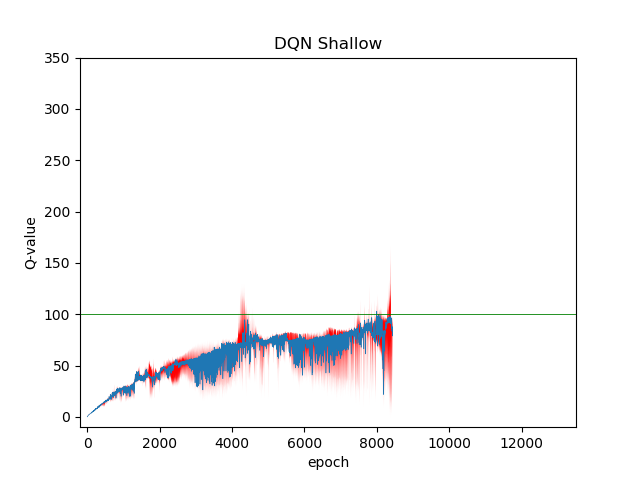
\includegraphics[width=.45\textwidth]{res/DQN_Shallow}} \quad
	\subfloat{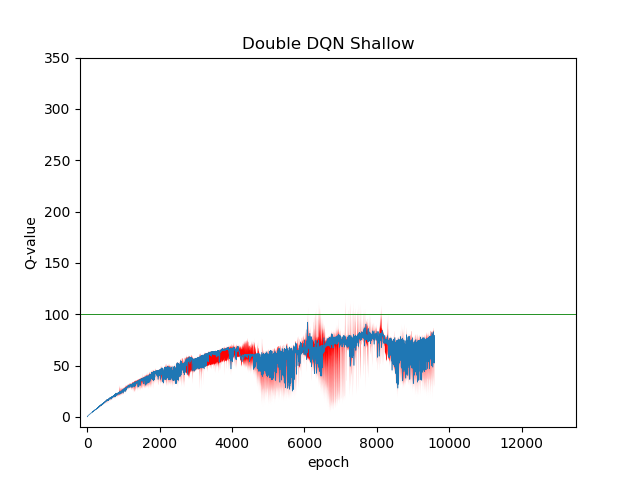
\includegraphics[width=.45\textwidth]{res/DoubleDQN_Shallow}} \\
	\subfloat{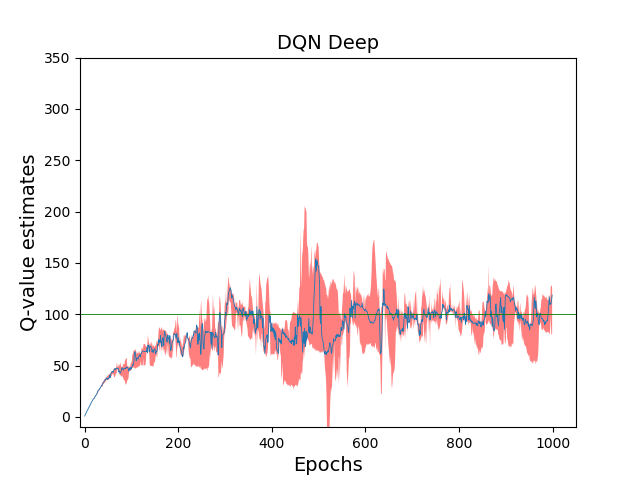
\includegraphics[width=.45\textwidth]{res/DQN_Deep}} \quad
	\subfloat{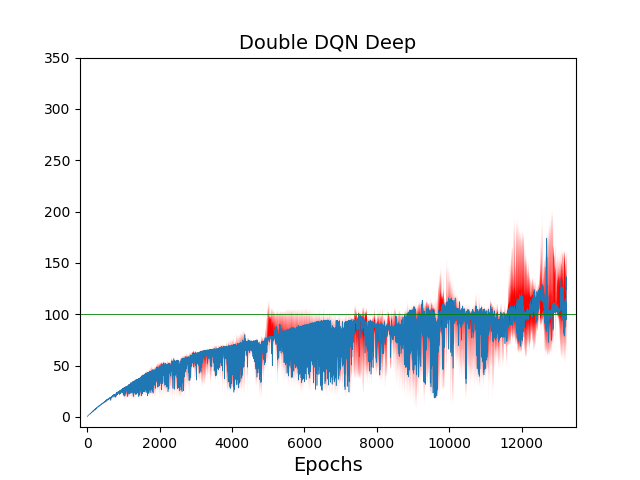
\includegraphics[width=.45\textwidth]{res/DoubleDQN_Deep}} \\
	
	%\subfloat[][\emph{Cascata}.]
	%{\includegraphics[width=.45\textwidth]{Cascata}} \quad
	%\subfloat[][\emph{Salita e discesa}.]
	%{\includegraphics[width=.45\textwidth]{SalitaDiscesa}}
	\caption{TODO}
	\label{fig:subfig}
\end{figure*}